\section{Doppelresonanzexperiment}
\subsection{Durchführung}
Für die Messung der Doppelresonanz ist das $\lambda$/4-Plättchen in den Strahlengang eingesetzt.
Mit dem Linearpolarisator (im Strahlengang nach dem $\lambda$/4-Plättchen) wird die
korrekte Win\-kel\-ein\-stel\-lung des $\lambda$/4-Plättchens gefunden,
indem die Schwankungen der transmittierten Intensität
bei Drehung des Polarisators minimiert werden.
Der RF-Sender auf der Zelle wird verwendet, um ein hochfrequentes Wechselfeld in das Rubidiumgas einzustrahlen.
Die Messung der Frequenz erfolgt mit dem Frequenzzähler im Versuchsaufbau.
An Spule 2 wird mit dem \emph{Instec function~generator} ein Sinussignal angelegt (siehe \autoref{img:dehmeltrf}),
das ein wechselndes Magnetfeld in Strahlrichtung erzeugt.
Mit der Photodiode wird die transmittierte Intensität der Strahlung gemessen,
die durch die Rubidiumzelle gelangt.
Auf \autoref{img:dehmeltrf} ist zu sehen, dass zusätzlich zu den erwarteten vier Doppelresonanz-Peaks pro
Periode der Magnetfeldmodulation zwei weitere Peaks pro Periode auftreten.
Diese Peaks bleiben bestehen, wenn das RF-Feld ausgeschaltet wird (siehe \autoref{img:dehmelt}) und
werden durch die Umkehr des Magnetfelds verursacht. Dies wird genauer in \autoref{sect:dehmelt} untersucht.

Zur Messung der Doppelresonanz wird ein weiteres zeitlich konstantes Magnetfeld in Strahlrichtung erzeugt,
indem ein Gleichstrom durch Spule 1 geschickt wird.
Durch die Variation dieses Stroms kann die Position der Absorptionspeaks der Doppelresonanz eingestellt werden
(siehe \autoref{img:rfwrong} und \autoref{img:rfcorrect}).
Für zwei verschiedene Radiofrequenzen (494\,kHz und 900\,kHz) und
zwei verschiedene LED-Ströme (62.9\,mA und 63.2\,mA) werden so die acht 
Werte für die Stromstärken bestimmt, bei denen die Absorptionspeaks äquidistant sind.
Dazu ist es notwendig, die Polung des Spulenstroms durch Umstecken der Kabel zu verändern.

Die Amplitude des Sinussignals zur Magnetfeldmodulation beträgt bei der Messung 0.16\,V und
die Temperatur des Peltierelements 33.9$^\circ$C.
Außerdem werden an Spule 4 86\,mA Gleichstrom angelegt, um das vertikale Magnetfeld zu kompensieren.
Die Höhe des Stroms wird durch Maximierung der Signalintensität bestimmt.




\begin{figure}[H]
\begin{center}
  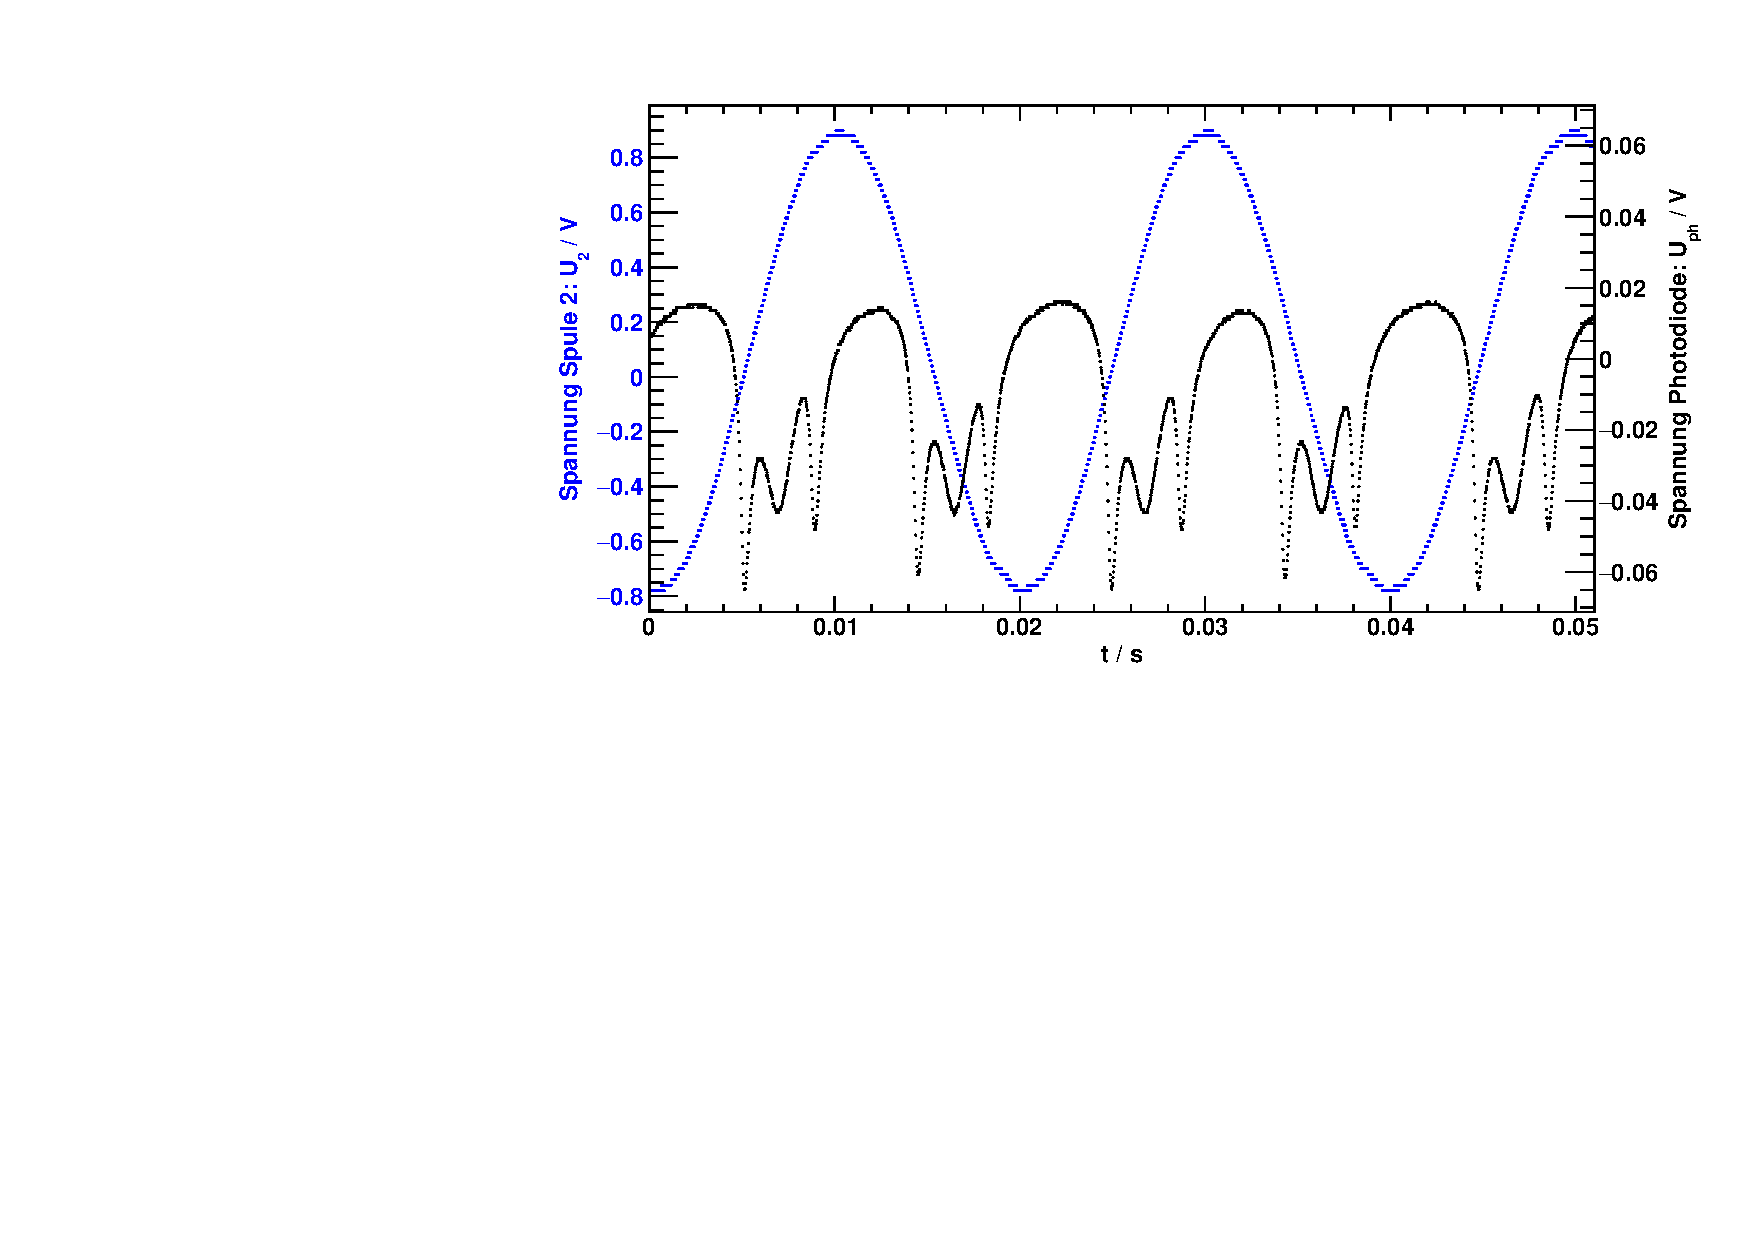
\includegraphics[width=\textwidth]{../img/part3/06.pdf}
  \caption{Starke Modulation des Magnetfelds in Strahlrichtung mit Spule 2 (schwarz).
   Im Photodiodensignal (rot) sind vier Doppelresonanz-Peaks sowie
   zwei Dehmelt-Peaks pro Modulationsperiode sichtbar.}
  \label{img:dehmeltrf}
\end{center}
\end{figure} 

\begin{figure}[H]
\begin{center}
  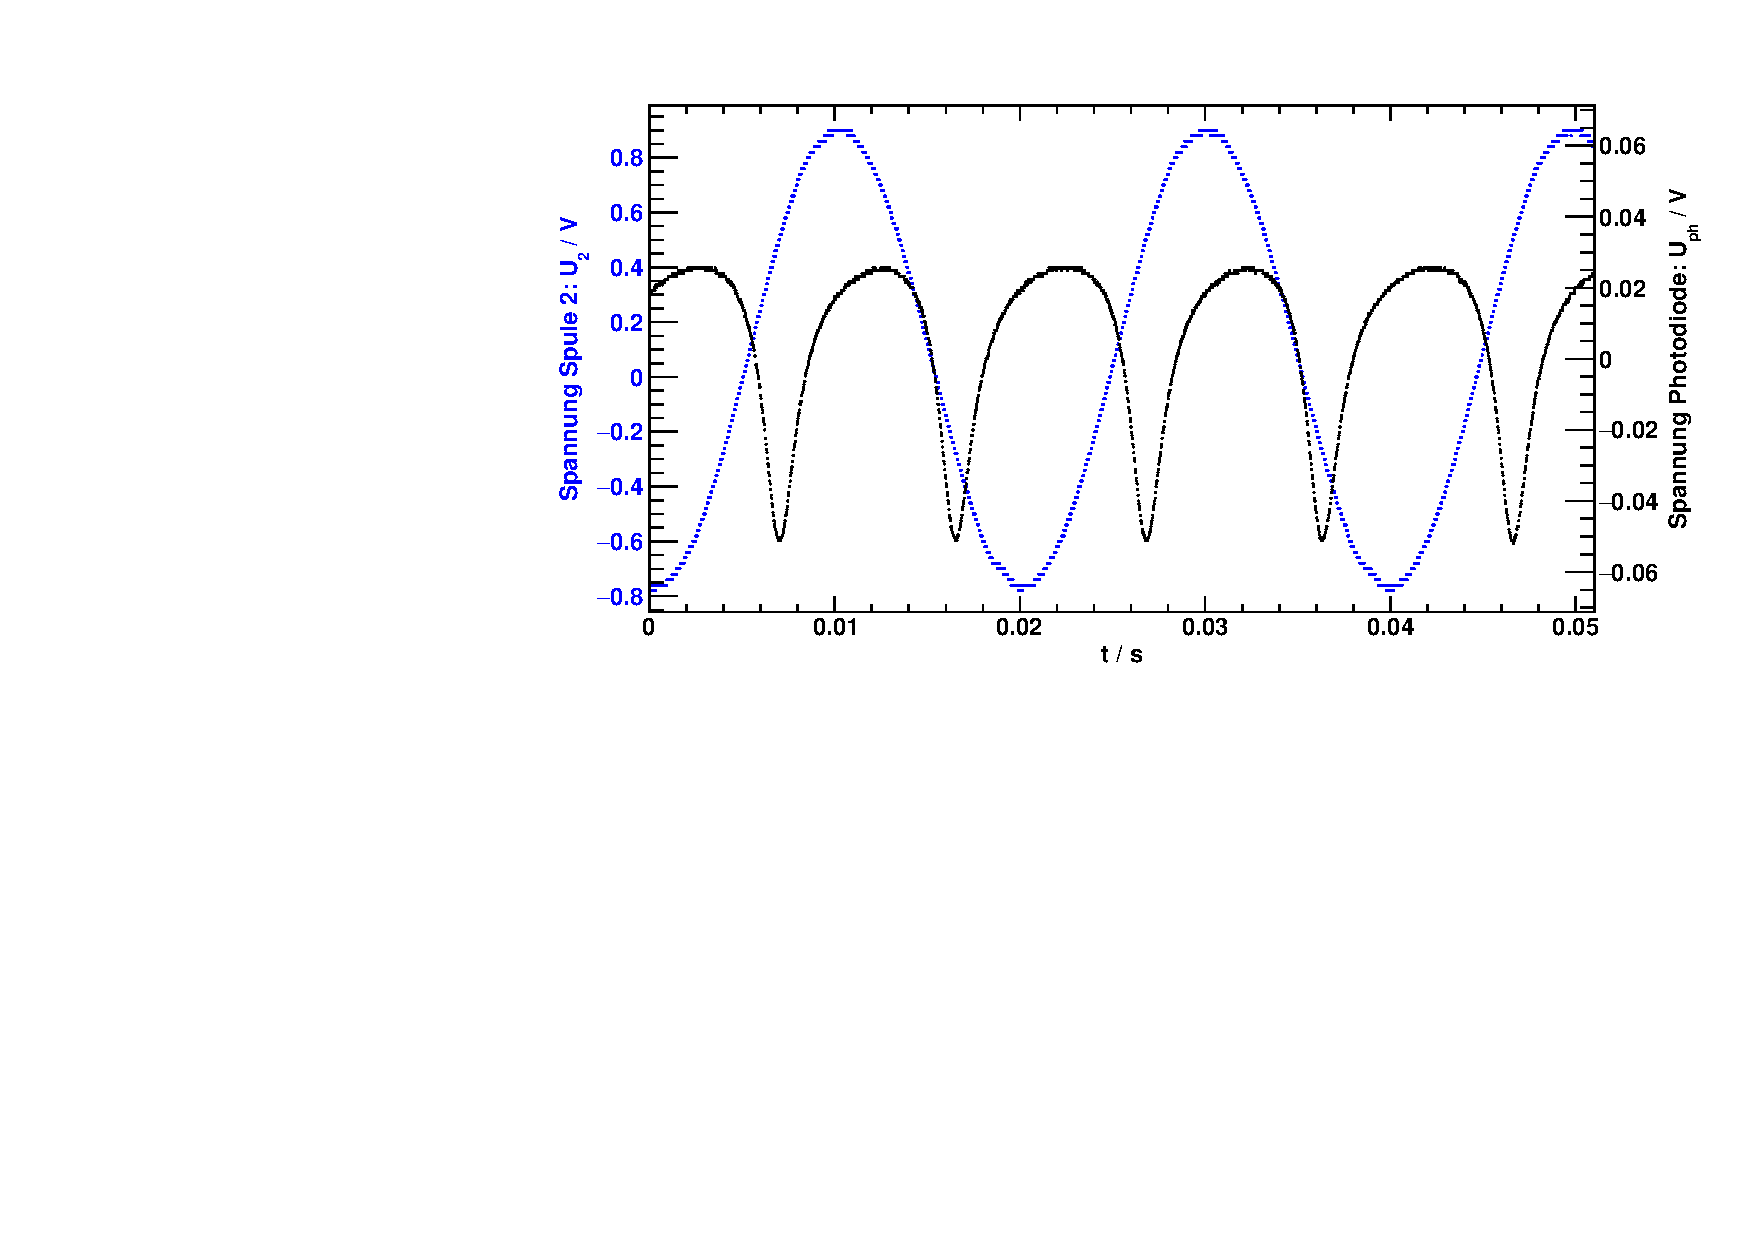
\includegraphics[width=\textwidth]{../img/part3/07.pdf}
  \caption{Gleiches Setup wie bei \autoref{img:dehmeltrf}, aber ohne RF-Signal.
  Die Dehmelt-Peaks sind weiterhin vorhanden.}
  \label{img:dehmelt}
\end{center}
\end{figure} 


\begin{figure}[H]
\begin{center}
  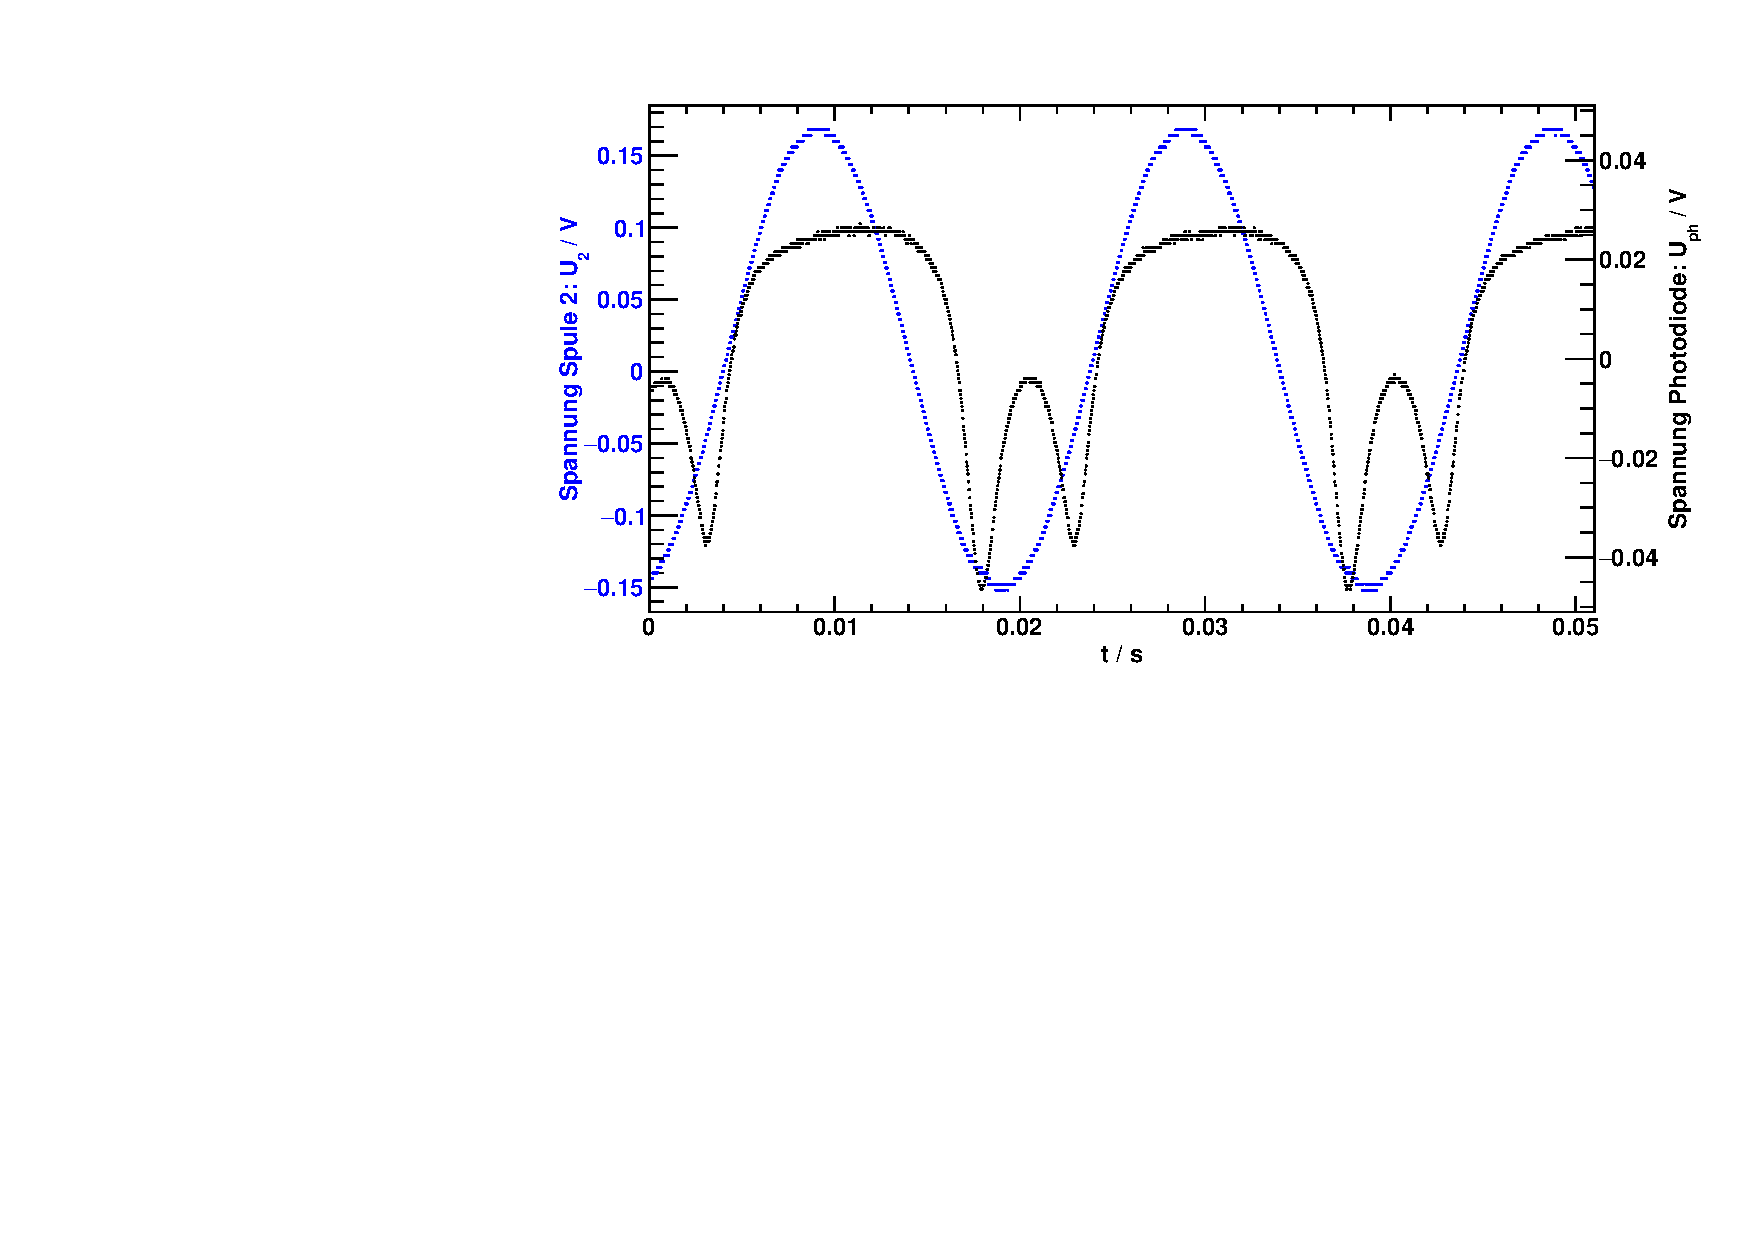
\includegraphics[width=\textwidth]{../img/part3/11.pdf}
  \caption{Doppelresonanz-Absorptionssignal: Falsche Einstellung des Gleichstroms in Spule 1,
  die Absorptionen sind nicht äquidistant.}
  \label{img:rfwrong}
\end{center}
\end{figure} 


\begin{figure}[H]
\begin{center}
  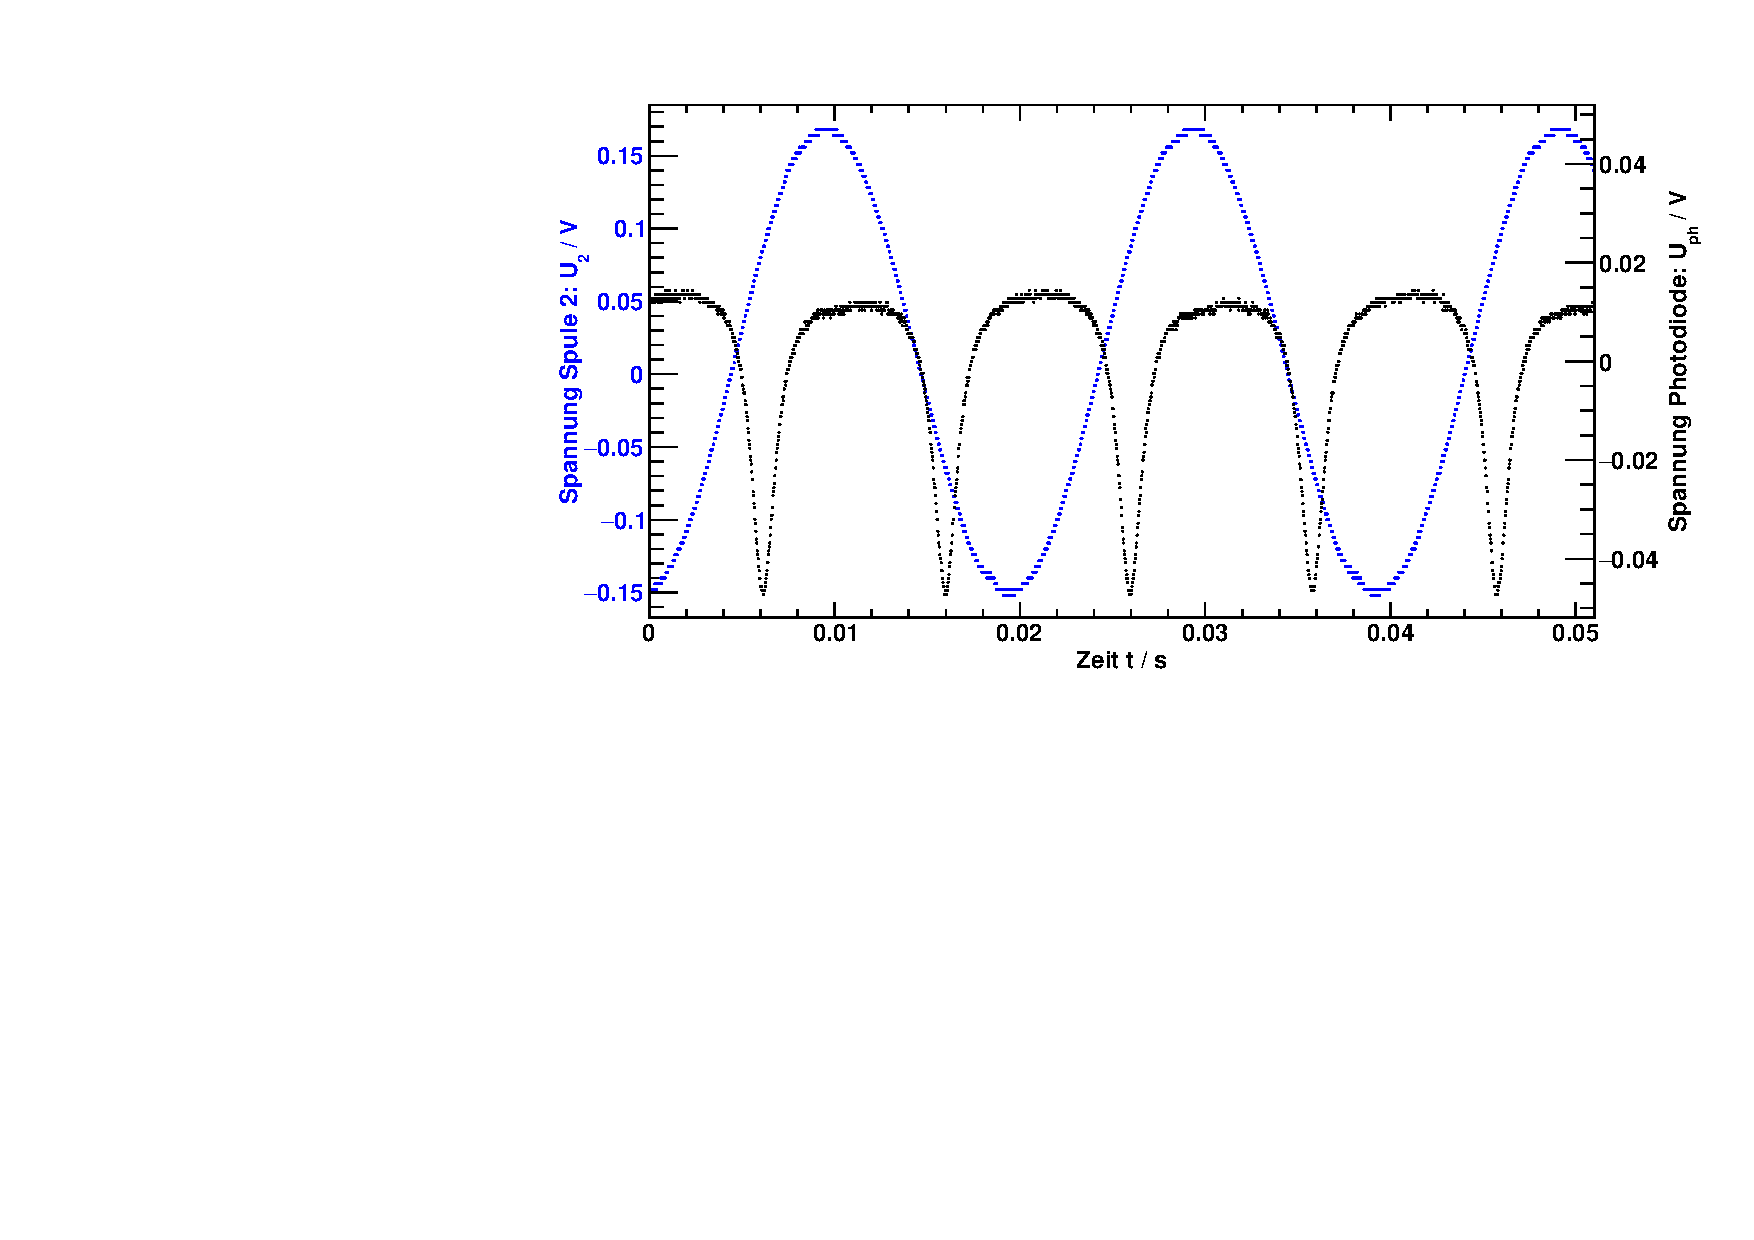
\includegraphics[width=\textwidth]{../img/part3/08.pdf}
  \caption{Doppelresonanz-Absorptionssignal: Korrekte Einstellung des Gleichstroms in Spule 1,
  die Absorptionen sind daher äquidistant.}
  \label{img:rfcorrect}
\end{center}
\end{figure} 

\subsection{Auswertung}
Berechnung Bhor, Bvert, I